<<<<<<< HEAD
How to world
=======
How to world . . .. . .\\
\\
A world is easily divided into different aspects. There are the sky, the oceans and the land. The land contain different terrain, with different types of ground and vegetation. There is a sun orbiting the world, casting rays of light and in the process creating reflections and indirectly making shadows.\\
\\
A procedural world is generated by carefully chosen algorithms. Our world is procedurally generated anew in a new unique constellation on every run, or a seed can be provided to generate specific worlds. The terrain is first formed, then the ground texturing and the vegetation, both dependent on properties of the terrain. The shadows depend on the sun and the waves on the terrain as well as on time itself.
>>>>>>> origin/master

\subsubsection{Sky}
The sky is achieved using a high-resolution texture of a sky mapped to a skybox. The mathematical location of the sun is placed as close as possible to the sun appearing in this texture. This gives shadows and shading a natural feel. The texture has been manually modified at the horizon to fade towards a shadowish gray color. The color is the same as the one objects are distance-fogged with. This makes the sky melt into the ocean in a very nice way. 

\subsubsection{Ocean}
// TODO  Tiger \\
<<<<<<< HEAD
Normal-mapped square

=======
Normal-mapped square with moving normal map. Makes the water glister/glitter from a far.\\\\
FIGURE(water that glister)
\\
Waves on the beaches is made by having several sinus waves aggregate horizontally to vary the wave fronts, and by having a sinus wave that control the vertical assent/decent of the waves.\\
\\
FIGURE(showing nice waves)

\newpage
>>>>>>> origin/master
\subsubsection{Terrain}
The terrain is generated by sampling a noise function and translating its value into a height for the current vertex. The noise in this case originates from a Simplex function. However, to get a realistically looking terrain one it is not sufficient to sample this function only once for every vertex.

Fractional Brownian Motion is calculated by sampling the Simplex function at different frequencies and calculating a weighted sum over the samples \cite{FracBrownMotion}. The result is a nice looking height map. 

\begin{figure}[H]
<<<<<<< HEAD

=======
>>>>>>> origin/master
\begin{subfigure}{.5\textwidth}
  \centering
  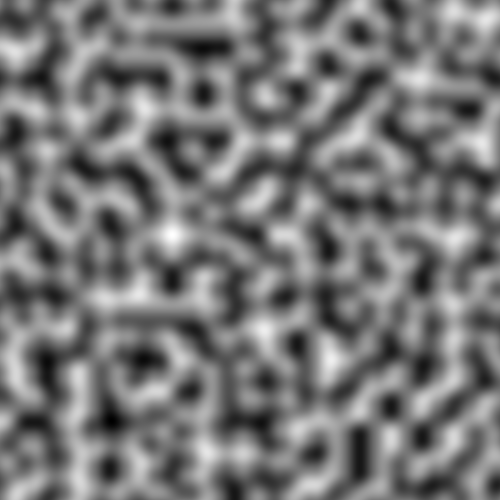
\includegraphics[width=0.9\linewidth]{images/Simplex.png}
  \caption{Height map generated from single-octave simplex noise}
  \label{fig:sub1}
\end{subfigure}%
\begin{subfigure}{.5\textwidth}
  \centering
  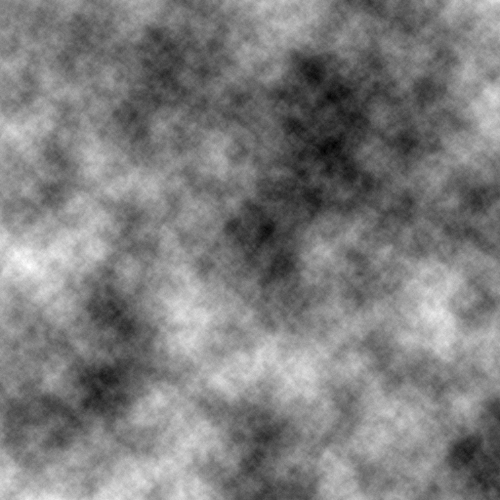
\includegraphics[width=0.9\linewidth]{images/FracBrownMotion.png}
  \caption{Height map generated with Fractional Brownian Motion}
  \label{fig:sub2}
\end{subfigure}
\caption[Noise comparison]{\textit{Comparison of noise functions}}
\label{fig:R_kitchen_example}
\end{figure}

<<<<<<< HEAD
=======
\subsubsection{Ground}
The ground is textured using a non-linear multi-texturing approach based on both altitude and terrain slope. Currently only three textures are used, one sandy, one grassy and one rocky. ... TODO: blah...\\
\\
FIGURE(comparison of texturing)
\\
FIGURE(comparison of texturing)
\\

>>>>>>> origin/master
\subsubsection{Content}
// TODO - Häger \\
Trees and rocks 





